\documentclass[8pt]{article}

\usepackage{fullpage}
\usepackage{tikz}
\usetikzlibrary{shapes.geometric, arrows}
\tikzstyle{startstop} = [rectangle, rounded corners, minimum height=0.5cm,text centered, draw=black, fill=red!30]
\tikzstyle{io} = [trapezium, trapezium left angle=70, trapezium right angle=110, minimum height=0.8cm, text centered, draw=black, fill=blue!30]
\tikzstyle{process} = [rectangle, minimum width=1cm, minimum height=1cm, text centered, draw=black, fill=orange!30]
\tikzstyle{decision} = [diamond, minimum width=1cm, minimum height=1cm, text centered, draw=black, fill=green!30]
\tikzstyle{arrow} = [thick,->,>=stealth]    
\tikzstyle{line} = [thick,-,>=stealth] 

\begin{document}

\title{ARM Checkpoint report}
\author{Fawwaz Abdullah (ffa20), Robert Buxton (rb419), \\Edward Hartley (ech120), Wojtek Sowinski (ws420) }

\maketitle

\section{Group Organisation}

\subsection{Work Distribution and Coordination}

In our initial group meeting, we found it difficult to divide work without having a
better handle on the problem as a whole. We had already agreed upon a style guide 
but realised there was still a bottleneck to overcome before we could code independently.
We split into two groups, with one coder and one observer each; one pair created general data
types and structures whilst the other implemented the overarching logic of the execute-decode-fetch cycle.
Communication was open between the groups to keep our concept of the overall project in sync. \\ \\
While we knew we would return to these central parts, the first drafts allowed us to split
further and each implement one category of instruction. The people with simpler instruction types
to implement could then work to create and improve central files such as a Makefile.
Finally the whole team collaborated to test and review each other's code and fix any bugs.

\subsection{Evaluation and Future Strategies}

Our primary method of communication is Discord where we have a video meeting at
11 am every day to discuss how the project is going and where we plan to go next.
We also communicate frequently in the chat which means that the team has a good
idea of the state of the project and any problems can be resolved promptly. \\ \\
What we would like to do in the future is find ways to reduce the amount of
downtime when team is waiting for bottlenecks to be completed. This can be resolved
by sending two members of the team ahead to decide useful function signatures and
data types so that the team can get straight to coding once the report is finished.

\section{Implementation}

\subsection{Emulator Data Structures}

\begin{itemize}

    \item \textbf{Program State} (\texttt{State}): A struct representing the 
    processor's current state. It holds a pointer to an array representing 
    all of the registers excluding the CPSR; a pointer to an array
    representing the processor's memory; the next instruction to be decoded; the 
    next instruction to be executed; flags representing whether decoded
    and fetched instructions are present; 
    the CPSR register and the last accessed memory address.
    
    \item \textbf{Decoded instruction} (\texttt{Instruction}): A struct representing
    a decoded instruction. It holds a condition code, a type referring to which type of 
    instruction it holds and lastly a strut representing the specific instruction to be executed.
    
    \item \textbf{Instruction types} There are 5 instruction types, the four specified 
    plus a halt type and they each have a struct
    representing them containing all the required data to execute them.

    
    \end{itemize}

\begin{minipage}{0.45\textwidth}
\subsection{Emulator Program Structure}

\begin{itemize}
    \item \texttt{decoder.c} \\ Decodes raw binary into one of the 5 instruction 
    types.
    \item \texttt{branch.c} \\ Simulates the branch instruction.
    \item \texttt{dataprocessing.c} \\ Simulates one of the ten data processing 
    instructions.
    \item \texttt{halt.c} \\  Halts the program.
    \item \texttt{multiply.c} \\ Simulates the multiply instruction.
    \item \texttt{singledatatransfer.c} \\ Simulates single data transfer instructions.
    \item \texttt{fetcher.c} \\ Fetches the next instruction from memory and
    increments the PC.
    \item \texttt{emulate.c} \\ initializes the processor and starts the fetch decode
    execute cycle on the binary file provided. 
    \item \texttt{printstate.c} \\ Prints the final state of the program after 
    halting.
\end{itemize}
\end{minipage}%
\hfill
\begin{minipage}{0.45\textwidth}

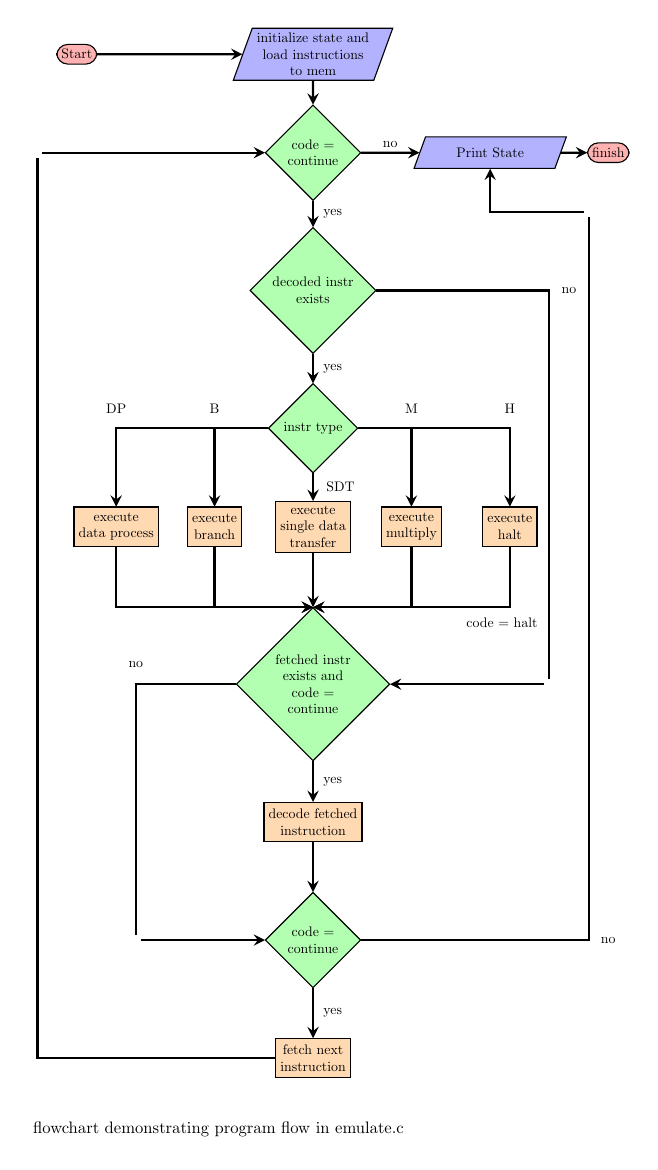
\begin{tikzpicture}[node distance=2cm]
    \node (start) [scale=0.5, startstop] at (0,0) {Start};
    \node (in1) [scale=0.5, align=center, io, right of=start, xshift=4cm] 
    {initialize state and \\ load instructions \\ to mem};
    \node (code) [scale=0.5, align=center, decision, below of=in1, yshift=-0.5cm] 
    {code = \\continue};
    \node (inv4) [scale=0.5, align=center ,right of=code, xshift = -9cm]
    {};
    \node (print) [scale=0.5, align=center, io, right of=code, xshift=2.5cm] 
    {Print State};
    \node (finish) [scale=0.5, startstop, right of=print, xshift=1cm] 
    {finish};
    \node (decoded?) [scale=0.5, align=center, decision, below of=code, yshift=-1.5cm] 
    {decoded instr \\ exists};
    \node (inv3) [scale=0.5, align=center ,right of=decoded?, xshift = 5cm, yshift = 2cm]
    {};
    \node (instr) [scale=0.5, align=center, decision, below of=decoded?, yshift=-1.5cm] 
    {instr type};
    \node (sdt) [scale=0.5, align=center, process, below of=instr, yshift=-0.5cm] 
    {execute \\ single data \\ transfer};
    \node (mult) [scale=0.5, align=center, process, right of=sdt, xshift = 0.5cm] 
    {execute \\ multiply};
    \node (halt) [scale=0.5, align=center, process, ,right of=mult, xshift = 0.5cm] 
    {execute \\ halt};
    \node (brch) [scale=0.5, align=center, process, left of=sdt, xshift = -0.5cm] 
    {execute \\ branch};
    \node (dp) [scale=0.5, align=center, process, left of=brch, xshift = -0.5cm] 
    {execute \\ data process};
    \node (fetched?) [scale=0.5, align=center, decision, below of=sdt, yshift=-2cm] 
    {fetched instr \\ exists and \\ code = \\continue};
    \node (inv1) [scale=0.5, align=center ,right of=fetched?, xshift = 4.0cm]
    {};
    \node (decoder) [scale=0.5, align=center, process, ,below of=fetched?, yshift = -1.5cm]
    {decode fetched \\ instruction};
    \node (tofetch) [scale=0.5, align=center, decision, below of=decoder, yshift=-1cm] 
    {code = \\continue};
    \node (inv2) [scale=0.5, align=center ,left of=tofetch, xshift = -2.5cm]
    {};
    \node (fetcher) [scale=0.5, align=center, process, ,below of=tofetch, yshift = -1cm]
    {fetch next \\ instruction};
    \node (desc) [scale = 0.6, align=center, below of=tofetch, yshift = -2cm, xshift = -2cm]
    {flowchart demonstrating program flow in emulate.c};

    \draw [arrow] (start) -- (in1);
    \draw [arrow] (in1) -- (code);
    \draw [arrow] (code) -- node[scale=0.5, yshift=0.2cm] {no} (print);
    \draw [arrow] (print) -- (finish);
    \draw [arrow] (code) -- node[scale=0.5, xshift=0.5cm] {yes} (decoded?);
    \draw [arrow] (decoded?) -- node[scale=0.5, xshift=0.5cm] {yes} (instr);
    \draw [line] (decoded?) -| node[scale=0.5, xshift=0.5cm] {no} (inv1);
    \draw [arrow] (inv1) -- (fetched?);
    \draw [arrow] (instr) -| node[scale=0.5, yshift=0.5cm] {DP} (dp);
    \draw [arrow] (instr) -| node[scale=0.5, yshift=0.5cm] {B} (brch);
    \draw [arrow] (instr) -- node[scale=0.5, xshift=0.7cm] {SDT} (sdt);
    \draw [arrow] (instr) -| node[scale=0.5, yshift=0.5cm] {M} (mult);
    \draw [arrow] (instr) -| node[scale=0.5, yshift=0.5cm] {H} (halt);
    \draw [arrow] (dp) |- (fetched?.north);
    \draw [arrow] (brch) |- (fetched?.north);
    \draw [arrow] (sdt) -- (fetched?.north);
    \draw [arrow] (mult) |- (fetched?.north);
    \draw [arrow] (halt) |- node[scale=0.5, xshift=-0.2cm ,yshift=-0.4cm] {code = halt} (fetched?.north);
    \draw [line] (fetched?) -| node[scale=0.5, yshift=0.5cm] {no} (inv2);
    \draw [arrow] (inv2) -- (tofetch);
    \draw [arrow] (fetched?) -- node[scale=0.5, xshift=0.5cm] {yes} (decoder);
    \draw [arrow] (decoder) -- (tofetch);
    \draw [line] (tofetch) -| node[scale=0.5, xshift=0.5cm] {no} (inv3);
    \draw [arrow] (inv3) -| (print);
    \draw [arrow] (tofetch) -- node[scale=0.5, xshift=0.5cm] {yes} (fetcher);
    \draw [arrow] (fetcher) -| (inv4) -- (code);
\end{tikzpicture}
\end{minipage}%


\subsection{Reusable elements for the assembler}
In our assembler, we plan to use many of the enum data types such as the
instruction types and exit-status codes; we also plan to reuse some of the
helper functions we created such as swap-endianess(). Due to the same 4 
instruction categories being present, we should be able to use a similar 
function pointer array as we did in emulate.c to call the correct function
per type of instruction.

\subsection{Future Tasks}
Parsing the assembly instructions may prove to be tedious, hopefully by discussing
our problems and working together to make robust helper functions we can reduce
this workload. Also, implementing the first pass of our planned two-pass assembly 
in such a way that symbols can be quickly found later may be challenging, we will
need to research appropiate data structures before committing to one.




\end{document}
